
%(BEGIN_QUESTION)
% Copyright 2011, Tony R. Kuphaldt, released under the Creative Commons Attribution License (v 1.0)
% This means you may do almost anything with this work of mine, so long as you give me proper credit

Anta at instrumentet i denne Wheatstone-brokretsen står ``helt i utslag'' selv når RTD-en er ved 0$^{o}$ C (når broen egentlig skal være i balanse), med polariteten over terminalene på indikerende voltmeter som vist:

$$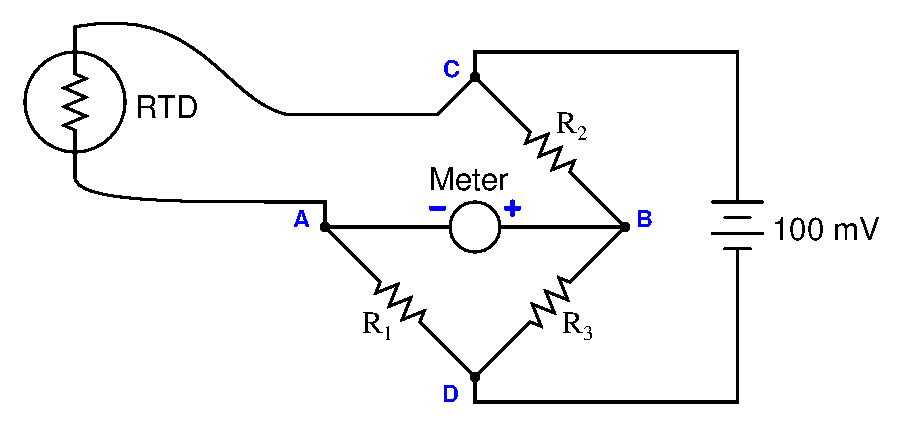
\includegraphics[width=15.5cm]{i01350x01.eps}$$

Vurder sannsynligheten for hver av de oppgitte feilene i denne kretsen. Betrakt hver feil separat (dvs. ingen sammenfallende feil), og avgjør om hver enkelt feil alene kan forklare {\it alle} målinger og symptomer i kretsen.

% Ingen blanklinjer er tillatt mellom linjer i en \halign-struktur!
% Jeg bruker kommentarer (%) i stedet, slik at TeX ikke feiler.

$$\vbox{\offinterlineskip
\halign{\strut
\vrule \quad\hfil # \ \hfil & 
\vrule \quad\hfil # \ \hfil & 
\vrule \quad\hfil # \ \hfil \vrule \cr
\noalign{\hrule}
%
% Første rad
{\bf Feil} & {\bf Mulig} & {\bf Umulig} \cr
%
\noalign{\hrule}
%
% Neste rad
$R_1$ har brudd (åpen krets) &  &  \cr
%
\noalign{\hrule}
%
% Neste rad
$R_2$ har brudd (åpen krets) &  &  \cr
%
\noalign{\hrule}
%
% Neste rad
$R_3$ har brudd (åpen krets) &  &  \cr
%
\noalign{\hrule}
%
% Neste rad
RTD har brudd (åpen krets) &  &  \cr
%
\noalign{\hrule}
%
% Neste rad
$R_1$ er kortsluttet &  &  \cr
%
\noalign{\hrule}
%
% Neste rad
$R_2$ er kortsluttet &  &  \cr
%
\noalign{\hrule}
%
% Neste rad
$R_3$ er kortsluttet &  &  \cr
%
\noalign{\hrule}
%
% Neste rad
RTD er kortsluttet &  &  \cr
%
\noalign{\hrule}
} % Slutt på \halign
}$$ % Slutt på \vbox

\underbar{file i01350}
%(END_QUESTION)





%(BEGIN_ANSWER)

% Ingen blanklinjer er tillatt mellom linjer i en \halign-struktur!
% Jeg bruker kommentarer (%) i stedet, slik at TeX ikke feiler.

$$\vbox{\offinterlineskip
\halign{\strut
\vrule \quad\hfil # \ \hfil & 
\vrule \quad\hfil # \ \hfil & 
\vrule \quad\hfil # \ \hfil \vrule \cr
\noalign{\hrule}
%
% Første rad
{\bf Feil} & {\bf Mulig} & {\bf Umulig} \cr
%
\noalign{\hrule}
%
% Neste rad
$R_1$ har brudd (åpen krets) &  & $\surd$ \cr
%
\noalign{\hrule}
%
% Neste rad
$R_2$ har brudd (åpen krets) &  & $\surd$ \cr
%
\noalign{\hrule}
%
% Neste rad
$R_3$ har brudd (åpen krets) & $\surd$ &  \cr
%
\noalign{\hrule}
%
% Neste rad
RTD har brudd (åpen krets) & $\surd$ &  \cr
%
\noalign{\hrule}
%
% Neste rad
$R_1$ er kortsluttet & $\surd$ &  \cr
%
\noalign{\hrule}
%
% Neste rad
$R_2$ er kortsluttet & $\surd$ &  \cr
%
\noalign{\hrule}
%
% Neste rad
$R_3$ er kortsluttet &  & $\surd$ \cr
%
\noalign{\hrule}
%
% Neste rad
RTD er kortsluttet &  & $\surd$ \cr
%
\noalign{\hrule}
} % Slutt på \halign
}$$ % Slutt på \vbox


%(END_ANSWER)





%(BEGIN_NOTES)

{\bf Dette spørsmålet er ment kun for eksamener, ikke for arbeidsark!}.

%(END_NOTES)

